\documentclass{standalone}
\begin{document}
\chapter{Pipeline}
The aim of this work of thesis is the implementation of an automated pipeline to predict the response to neoadjuvant chemo-radiotherapy of patients affected by colorectal cancer by using radiomic features.
\\
The work was developed and validated on MRI scans provided by IRCCS Sant’Orsola-Malpighi Polyclinic.

\begin{figure}[htp]

    \centering
    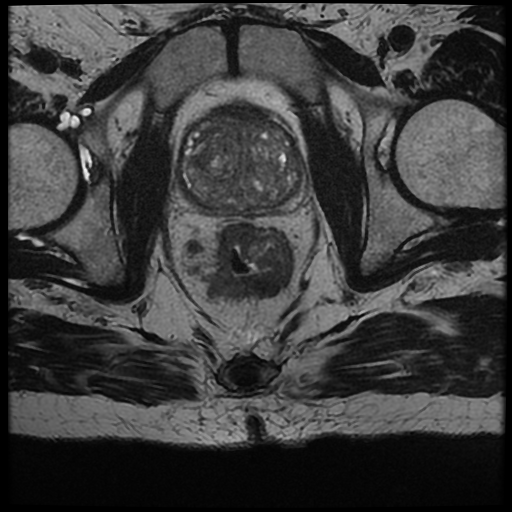
\includegraphics[width=.32\textwidth]{../images/11.png} \hfill
    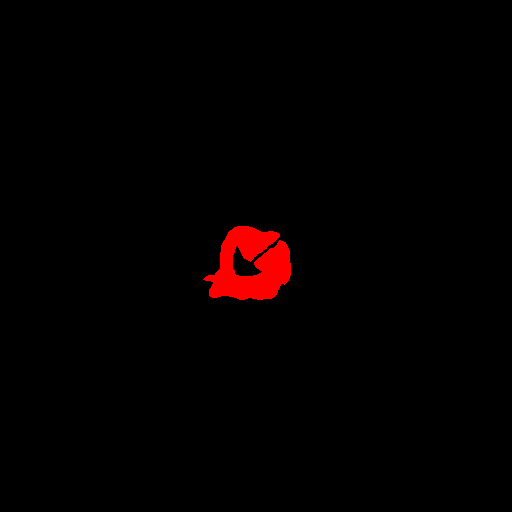
\includegraphics[width=.32\textwidth]{../images/11_mask_red.png} \hfill
    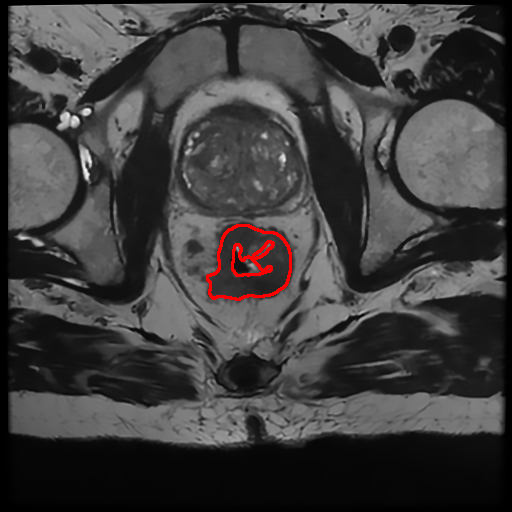
\includegraphics[width=.32\textwidth]{../images/11_cont.png}
    
    \caption{\textit{ From left to right:} the original MR image of a patient affected by colorectal cancer;
    the segmentation mask of the tumor region obtained from manual annotations made by expert radiologists; the same image with identified tumor area.}
    \label{comparison}
    
    \end{figure}

The starting point is the MRI scans. 
Firstly, I started with the visualization and the pre-processing of the scans.
The pre-processing consists of a technique to remove noise which could be a potential source of false positives and gamma correction to increase the contrast of the images.
\\
The work was then split into two main frameworks: \textit{segmentation} and \textit{radiomics}.
The basic idea was to train a Convolutional Neural Network like U-Net, for the segmentation of the images.
The training process was supervised exploiting segmentation masks of the tumor regions.
The masks come from manual annotations made by expert radiologists.
\\
Once trained, the Convolutional Neural Network model was applied to perform the segmentation of the images to get the tumor regions for each patient.
\\
The next step is the extraction of radiomic features.
They are extracted from the obtained segmented regions.
The features are then analyzed to implement a model for the prediction of response.
The prediction is based on the Tumor Regression Grade (TRG), which gives an evaluation of how much the chemo-radiotherapy was effective.
\\
The workflow of the developed pipeline can be seen in Figure \ref{workflow}
\begin{figure}[htp]

    \centering
    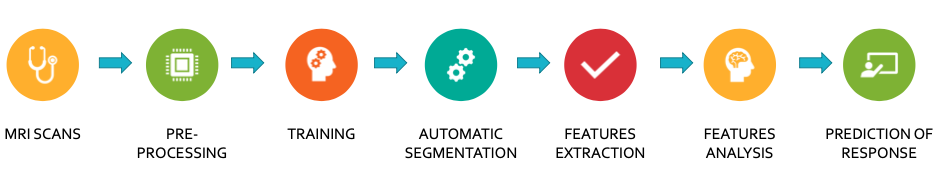
\includegraphics[width=\textwidth]{../images/finalworkflow.png}
    
    \caption{Workflow of the developed pipeline. The starting point is the MRI scans. Then, the images are pre-processed for the training of a Convolutional Neural Network model. After the segmentation of the images, radiomic features are extracted from the obtained segmented regions. They are analyzed to implement a model for the prediction of response based on the Tumor Regression Grade (TRG).}
    \label{workflow}
    
    \end{figure}


Obviously, the final pipeline structure does not involve a learning process and a feature analysis step since the models are already implemented.
As consequence, the final structure of the pipeline looks like in the following Figure \ref{pipeline}
\begin{figure}[ht]

    \centering
    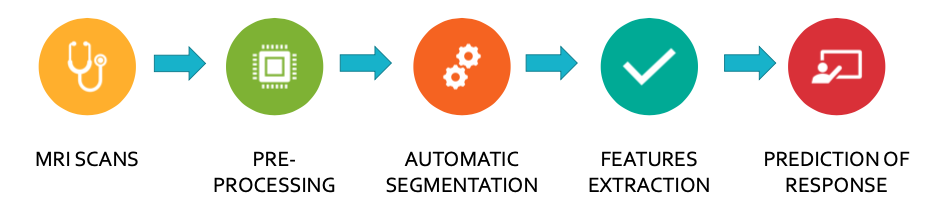
\includegraphics[width=\textwidth]{../images/finalpipeline.png}
    
    \caption{Final pipeline structure. The MRI scans are pre-processed with the non-local means algorithm and gamma correction to remove possible noise sources and improve the image contrast, respectively. Then, the segmentation is achieved by the trained CNN model. After the segmentation, radiomic features are extracted. Finally, the prediction of response is obtained by the implemented model.}
    \label{pipeline}
    
    \end{figure}

\end{document}